\documentclass[conference,letterpaper]{IEEEtran}
\IEEEoverridecommandlockouts
\usepackage{cite}
\usepackage{amsmath,amssymb}
\usepackage{graphicx}
\usepackage{booktabs}
\usepackage{array}
\usepackage{xcolor}
\usepackage{url}
\usepackage[hidelinks]{hyperref}

% Every result below is a macro generated from the evaluation outputs
% (make_numbers.py -> numbers.tex for CHB-MIT, make_numbers_s2.py -> numbers_s2.tex for SeizeIT2).
% AUTO-GENERATED by make_numbers.py — do not edit by hand
% source: ../final2
\newcommand{\Pilot}{0}
\newcommand{\PilotNote}{}
\newcommand{\NSubj}{23}
\newcommand{\NRec}{160}
\newcommand{\NSz}{194}
\newcommand{\NHours}{220}
\newcommand{\NColdStart}{15}
\newcommand{\NRecAll}{165}
\newcommand{\NSzAll}{198}
\newcommand{\NHoursAll}{225}
\newcommand{\PyBSens}{5.7\%}
\newcommand{\PyBDet}{11}
\newcommand{\PyBCI}{2--12\%}
\newcommand{\PyBMacro}{10.0\%}
\newcommand{\PyBMacroCI}{3--18\%}
\newcommand{\PyBFAh}{0.32}
\newcommand{\PyBFAday}{8}
\newcommand{\PyBFACI}{0.20--0.48}
\newcommand{\PyBLat}{26.3}
\newcommand{\PyASens}{21.1\%}
\newcommand{\PyADet}{41}
\newcommand{\PyACI}{14--29\%}
\newcommand{\PyAMacro}{25.4\%}
\newcommand{\PyAMacroCI}{15--36\%}
\newcommand{\PyAFAh}{2.82}
\newcommand{\PyAFAday}{68}
\newcommand{\PyAFACI}{2.00--3.86}
\newcommand{\PyALat}{28.4}
\newcommand{\FwBSens}{75.3\%}
\newcommand{\FwBDet}{146}
\newcommand{\FwBCI}{60--94\%}
\newcommand{\FwBMacro}{87.6\%}
\newcommand{\FwBMacroCI}{79--95\%}
\newcommand{\FwBFAh}{18.29}
\newcommand{\FwBFAday}{439}
\newcommand{\FwBFACI}{15.19--21.21}
\newcommand{\FwBLat}{14.5}
\newcommand{\DevASens}{52.1\%}
\newcommand{\DevADet}{101}
\newcommand{\DevACI}{36--74\%}
\newcommand{\DevAMacro}{68.6\%}
\newcommand{\DevAMacroCI}{54--82\%}
\newcommand{\DevAFAh}{0.97}
\newcommand{\DevAFAday}{23}
\newcommand{\DevAFACI}{0.71--1.31}
\newcommand{\DevALat}{22.0}
\newcommand{\DevBSens}{41.8\%}
\newcommand{\DevBDet}{81}
\newcommand{\DevBCI}{26--65\%}
\newcommand{\DevBMacro}{59.5\%}
\newcommand{\DevBMacroCI}{44--74\%}
\newcommand{\DevBFAh}{0.46}
\newcommand{\DevBFAday}{11}
\newcommand{\DevBFACI}{0.25--0.77}
\newcommand{\DevBLat}{23.0}
\newcommand{\DevCSens}{28.4\%}
\newcommand{\DevCDet}{55}
\newcommand{\DevCCI}{15--49\%}
\newcommand{\DevCMacro}{46.1\%}
\newcommand{\DevCMacroCI}{30--62\%}
\newcommand{\DevCFAh}{0.16}
\newcommand{\DevCFAday}{4}
\newcommand{\DevCFACI}{0.05--0.32}
\newcommand{\DevCLat}{29.0}
\newcommand{\LlASens}{25.3\%}
\newcommand{\LlADet}{49}
\newcommand{\LlACI}{15--42\%}
\newcommand{\LlAMacro}{40.1\%}
\newcommand{\LlAMacroCI}{26--55\%}
\newcommand{\LlAFAh}{1.04}
\newcommand{\LlAFAday}{25}
\newcommand{\LlAFACI}{0.72--1.35}
\newcommand{\LlALat}{32.0}
\newcommand{\LlBSens}{21.6\%}
\newcommand{\LlBDet}{42}
\newcommand{\LlBCI}{11--38\%}
\newcommand{\LlBMacro}{35.8\%}
\newcommand{\LlBMacroCI}{21--50\%}
\newcommand{\LlBFAh}{0.35}
\newcommand{\LlBFAday}{8}
\newcommand{\LlBFACI}{0.23--0.51}
\newcommand{\LlBLat}{24.5}
\newcommand{\FuASens}{40.2\%}
\newcommand{\FuADet}{78}
\newcommand{\FuACI}{24--64\%}
\newcommand{\FuAMacro}{56.0\%}
\newcommand{\FuAMacroCI}{41--70\%}
\newcommand{\FuAFAh}{0.96}
\newcommand{\FuAFAday}{23}
\newcommand{\FuAFACI}{0.67--1.27}
\newcommand{\FuALat}{21.5}
\newcommand{\TwoDevASens}{52.1\%}
\newcommand{\TwoDevADet}{101}
\newcommand{\TwoDevACI}{36--74\%}
\newcommand{\TwoDevAMacro}{68.6\%}
\newcommand{\TwoDevAMacroCI}{54--82\%}
\newcommand{\TwoDevAFAh}{0.95}
\newcommand{\TwoDevAFAday}{23}
\newcommand{\TwoDevAFACI}{0.69--1.31}
\newcommand{\TwoDevALat}{23.0}
\newcommand{\TwoDevBSens}{38.1\%}
\newcommand{\TwoDevBDet}{74}
\newcommand{\TwoDevBCI}{24--61\%}
\newcommand{\TwoDevBMacro}{57.3\%}
\newcommand{\TwoDevBMacroCI}{41--73\%}
\newcommand{\TwoDevBFAh}{0.37}
\newcommand{\TwoDevBFAday}{9}
\newcommand{\TwoDevBFACI}{0.23--0.55}
\newcommand{\TwoDevBLat}{27.0}
\newcommand{\NeASens}{52.1\%}
\newcommand{\NeADet}{101}
\newcommand{\NeACI}{36--74\%}
\newcommand{\NeAMacro}{68.6\%}
\newcommand{\NeAMacroCI}{54--82\%}
\newcommand{\NeAFAh}{0.97}
\newcommand{\NeAFAday}{23}
\newcommand{\NeAFACI}{0.71--1.31}
\newcommand{\NeALat}{22.0}
\newcommand{\NeBSens}{41.8\%}
\newcommand{\NeBDet}{81}
\newcommand{\NeBCI}{26--65\%}
\newcommand{\NeBMacro}{59.5\%}
\newcommand{\NeBMacroCI}{44--74\%}
\newcommand{\NeBFAh}{0.46}
\newcommand{\NeBFAday}{11}
\newcommand{\NeBFACI}{0.25--0.77}
\newcommand{\NeBLat}{23.0}
\newcommand{\DevASensWarm}{54.2\%}
\newcommand{\DevASzWarm}{179}
\newcommand{\DevBSensWarm}{43.6\%}
\newcommand{\DevBSzWarm}{179}
\newcommand{\DevAR}{1.25}
\newcommand{\DevAD}{20}
\newcommand{\DevAModeCount}{22}
\newcommand{\DevAFolds}{23}
\newcommand{\DevBR}{1.5}
\newcommand{\DevBD}{20}
\newcommand{\DevBModeCount}{20}
\newcommand{\DevBFolds}{23}
\newcommand{\NestedDev}{69}
\newcommand{\NestedAll}{69}
\newcommand{\PyBNull}{1.6\%}
\newcommand{\PyBNullNF}{3.1\%}
\newcommand{\PyBNullP}{$p{=}1{\times}10^{-3}$}
\newcommand{\PyANull}{12.8\%}
\newcommand{\PyANullNF}{16.5\%}
\newcommand{\PyANullP}{$p{=}0.002$}
\newcommand{\FwBNull}{56.6\%}
\newcommand{\FwBNullNF}{61.3\%}
\newcommand{\FwBNullP}{$p{=}1{\times}10^{-3}$}
\newcommand{\DevANull}{6.5\%}
\newcommand{\DevANullNF}{9.3\%}
\newcommand{\DevANullP}{$p{=}1{\times}10^{-3}$}
\newcommand{\DevBNull}{3.9\%}
\newcommand{\DevBNullNF}{6.2\%}
\newcommand{\DevBNullP}{$p{=}1{\times}10^{-3}$}
\newcommand{\LlANull}{4.8\%}
\newcommand{\LlANullNF}{7.2\%}
\newcommand{\LlANullP}{$p{=}1{\times}10^{-3}$}
\newcommand{\NPerm}{1000}
\newcommand{\ShipNullMaxP}{0.002}
\newcommand{\TestDevPyP}{$p{=}6{\times}10^{-5}$}
\newcommand{\TestDevPyBetter}{21}
\newcommand{\TestDevPyWorse}{0}
\newcommand{\TestDevPyTies}{2}
\newcommand{\TestDevPyN}{23}
\newcommand{\TestDevPyAnyP}{$p{=}7{\times}10^{-5}$}
\newcommand{\TestDevPyAnyBetter}{20}
\newcommand{\TestDevPyAnyWorse}{1}
\newcommand{\TestDevPyAnyTies}{2}
\newcommand{\TestDevPyAnyN}{23}
\newcommand{\TestDevLlP}{$p{=}7{\times}10^{-4}$}
\newcommand{\TestDevLlBetter}{15}
\newcommand{\TestDevLlWorse}{0}
\newcommand{\TestDevLlTies}{8}
\newcommand{\TestDevLlN}{23}
\newcommand{\FoldDevPy}{7}
\newcommand{\AucLL}{0.70}
\newcommand{\AucLLCase}{0.79}
\newcommand{\AucDAR}{0.51}
\newcommand{\AucDARCase}{0.58}
\newcommand{\AucHFE}{0.40}
\newcommand{\AucHFECase}{0.41}
\newcommand{\AucFW}{0.70}
\newcommand{\AucFWCase}{0.83}
\newcommand{\ArtIctal}{0.01\%}
\newcommand{\ArtInter}{0.01\%}
\newcommand{\PyBSensLowGain}{0.0\%}
\newcommand{\PyBSensHighGain}{13.4\%}
\newcommand{\PyBFAhLowGain}{0.24}
\newcommand{\PyBFAhHighGain}{1.59}
\newcommand{\FwBFAhLowGain}{7.36}
\newcommand{\FwBFAhHighGain}{24.37}
\newcommand{\MainTableBody}{%
Analyzer, BLACKOUT (shipped) & 11/194 & 5.7\% [2--12] & 10.0\% & 0.32 & 26.3 & 1.6\% \\
Analyzer, any alarm (shipped) & 41/194 & 21.1\% [14--29] & 25.4\% & 2.82 & 28.4 & 12.8\% \\
Firmware, BLACKOUT (shipped) & 146/194 & 75.3\% [60--94] & 87.6\% & 18.29 & 14.5 & 56.6\% \\
\midrule
LL-BR, $\le$1 FA/h & 49/194 & 25.3\% [15--42] & 40.1\% & 1.04 & 32.0 & 4.8\% \\
FUSE-BR, $\le$1 FA/h & 78/194 & 40.2\% [24--64] & 56.0\% & 0.96 & 21.5 & -- \\
\textbf{DEV-BR, $\le$1 FA/h} & 101/194 & 52.1\% [36--74] & 68.6\% & 0.97 & 22.0 & 6.5\% \\
\textbf{DEV-BR, $\le$0.5 FA/h} & 81/194 & 41.8\% [26--65] & 59.5\% & 0.46 & 23.0 & 3.9\% \\
\textbf{DEV-BR, $\le$0.2 FA/h} & 55/194 & 28.4\% [15--49] & 46.1\% & 0.16 & 29.0 & -- \\
}
\newcommand{\AltBestOneSens}{51.0\%}
\newcommand{\AltBestHalfSens}{44.3\%}
\newcommand{\GbmOneSens}{47.9\%}
\newcommand{\GbmHalfSens}{44.3\%}
\newcommand{\GbmHalfBetter}{4}
\newcommand{\GbmHalfWorse}{2}
\newcommand{\GbmHalfP}{$p{=}0.25$}
\newcommand{\AblationTableBody}{%
\textbf{reference} (300 s, lag 30 s, median) & 52.1\% / 0.97 & 41.8\% / 0.46 \\
no lag (0 s) & 50.5\% / 0.79 & 34.5\% / 0.42 \\
lag 10 s & 51.0\% / 0.87 & 40.7\% / 0.45 \\
lag 60 s & 47.9\% / 0.93 & 38.7\% / 0.46 \\
window 60 s & 50.5\% / 0.94 & 43.3\% / 0.45 \\
window 120 s & 53.1\% / 0.88 & 38.1\% / 0.43 \\
window 600 s & 41.2\% / 0.94 & 34.0\% / 0.47 \\
mean instead of median & 50.0\% / 0.78 & 41.2\% / 0.35 \\
no normalization (absolute) & 32.5\% / 0.83 & 30.4\% / 0.42 \\
\midrule
k-of-n persistence & 43.3\% / 0.95 & 36.6\% / 0.38 \\
dual time-scale rule & 51.0\% / 1.01 & 42.8\% / 0.49 \\
baseline carried across files & 48.5\% / 0.97 & 41.8\% / 0.46 \\
log.\ regression, firmware features & 43.3\% / 1.03 & 35.1\% / 0.44 \\
log.\ regression, all features & 43.8\% / 0.90 & 38.7\% / 0.47 \\
boosted trees, all features & 47.9\% / 1.01 & 44.3\% / 0.50 \\
}
\newcommand{\AblAbsSens}{32.5\%}
\newcommand{\AblLagZeroSensB}{34.5\%}
\newcommand{\AblMeanSens}{50.0\%}
\newcommand{\AblWinLongSens}{41.2\%}
\newcommand{\DevSensOne}{44.4\%}
\newcommand{\SecLlPOne}{$p{=}0.061$}
\newcommand{\SecNestedDevOne}{67}
\newcommand{\DevSensTwo}{39.9\%}
\newcommand{\SecLlPTwo}{$p{=}0.055$}
\newcommand{\SecNestedDevTwo}{63}
\newcommand{\SecondaryTableBody}{%
FP1-F7 & 28.3\% / 4.01 & 77.3\% / 24.42 & 33.8\% / 0.95 & 44.4\% / 0.78 \\
FP2-F8 & 29.3\% / 3.83 & 82.8\% / 24.79 & 27.3\% / 0.89 & 39.9\% / 0.86 \\
}
\newcommand{\HwAvailable}{1}
\newcommand{\HwTableBody}{%
$\times$500 & 0.00\% & 52.1\% / 0.98 & 47.9\% / 0.94 & 51.5\% / 7.36 \\
$\times$1000 (ref.) & 0.00\% & 52.1\% / 0.95 & 52.1\% / 0.97 & 75.3\% / 18.29 \\
$\times$2000 & 0.01\% & 52.1\% / 0.97 & 50.0\% / 0.96 & 86.1\% / 24.37 \\
$\times$1000, LM358 clip & 0.52\% & 51.5\% / 0.97 & 48.5\% / 0.96 & 73.2\% / 18.01 \\
$\times$2000, LM358 clip & 2.69\% & 50.0\% / 0.93 & 50.0\% / 0.93 & 82.0\% / 23.09 \\
$\times$1000, 3.1-V ADC & 0.00\% & 52.1\% / 0.96 & 50.5\% / 0.98 & 78.9\% / 19.22 \\
$\times$1000, 167-Hz loop & 0.00\% & 51.5\% / 0.95 & 51.5\% / 0.96 & 45.9\% / 14.74 \\
}
\newcommand{\HwFixR}{1.25}
\newcommand{\HwFixD}{20}
\newcommand{\HwDevSensMin}{50.0\%}
\newcommand{\HwDevSensMax}{52.1\%}
\newcommand{\HwDevFAMin}{0.93}
\newcommand{\HwDevFAMax}{0.98}
\newcommand{\HwFwSensMin}{45.9\%}
\newcommand{\HwFwSensMax}{86.1\%}
\newcommand{\HwFwFAMin}{7.36}
\newcommand{\HwFwFAMax}{24.37}
\newcommand{\HwGainSens}{52.1\%}
\newcommand{\HwClipSat}{2.7\%}
\newcommand{\HwClipSens}{50.0\%}

% AUTO-GENERATED by make_numbers_s2.py — do not edit by hand
\newcommand{\SNSubj}{125}
\newcommand{\SNRuns}{2850}
\newcommand{\SNSz}{883}
\newcommand{\SHours}{11{,}626}
\newcommand{\SMovMissing}{386}
\newcommand{\SNMotor}{371}
\newcommand{\SNNonMotor}{324}
\newcommand{\SNFBTC}{55}
\newcommand{\SNOther}{133}
\newcommand{\SFwTarget}{7.01}
\newcommand{\SNSleep}{367}
\newcommand{\SFwSens}{57.0\%}
\newcommand{\SFwDet}{503}
\newcommand{\SFwFAh}{7.01}
\newcommand{\SFwFAday}{168.2}
\newcommand{\SFwMacro}{59.5\%}
\newcommand{\SFwCI}{47--65\%}
\newcommand{\SFwLat}{18.1}
\newcommand{\SFwMot}{55.3\%}
\newcommand{\SFwNonMot}{54.6\%}
\newcommand{\SFwFBTC}{87.3\%}
\newcommand{\SFwSleep}{64.0\%}
\newcommand{\SFwAwake}{58.0\%}
\newcommand{\SFwNull}{29.9\%}
\newcommand{\SFwNullP}{$p{=}0.005$}
\newcommand{\SEegASens}{33.1\%}
\newcommand{\SEegADet}{292}
\newcommand{\SEegAFAh}{0.93}
\newcommand{\SEegAFAday}{22.3}
\newcommand{\SEegAMacro}{47.6\%}
\newcommand{\SEegACI}{23--44\%}
\newcommand{\SEegALat}{40.0}
\newcommand{\SEegAMot}{41.8\%}
\newcommand{\SEegANonMot}{16.0\%}
\newcommand{\SEegAFBTC}{92.7\%}
\newcommand{\SEegASleep}{32.2\%}
\newcommand{\SEegAAwake}{36.2\%}
\newcommand{\SEegANull}{4.7\%}
\newcommand{\SEegANullP}{$p{=}0.005$}
\newcommand{\SEegBSens}{24.0\%}
\newcommand{\SEegBDet}{212}
\newcommand{\SEegBFAh}{0.47}
\newcommand{\SEegBFAday}{11.3}
\newcommand{\SEegBMacro}{36.4\%}
\newcommand{\SEegBCI}{15--35\%}
\newcommand{\SEegBLat}{44.0}
\newcommand{\SEegBMot}{28.6\%}
\newcommand{\SEegBNonMot}{9.3\%}
\newcommand{\SEegBFBTC}{92.7\%}
\newcommand{\SEegBSleep}{23.7\%}
\newcommand{\SEegBAwake}{25.4\%}
\newcommand{\SEegBNull}{2.8\%}
\newcommand{\SEegBNullP}{$p{=}0.005$}
\newcommand{\SEegCSens}{14.4\%}
\newcommand{\SEegCDet}{127}
\newcommand{\SEegCFAh}{0.22}
\newcommand{\SEegCFAday}{5.3}
\newcommand{\SEegCMacro}{24.9\%}
\newcommand{\SEegCCI}{8--24\%}
\newcommand{\SEegCLat}{47.0}
\newcommand{\SEegCMot}{13.7\%}
\newcommand{\SEegCNonMot}{2.8\%}
\newcommand{\SEegCFBTC}{89.1\%}
\newcommand{\SEegCSleep}{16.1\%}
\newcommand{\SEegCAwake}{13.1\%}
\newcommand{\SMovASens}{28.3\%}
\newcommand{\SMovADet}{250}
\newcommand{\SMovAFAh}{1.00}
\newcommand{\SMovAFAday}{24.0}
\newcommand{\SMovAMacro}{42.8\%}
\newcommand{\SMovACI}{22--36\%}
\newcommand{\SMovALat}{33.0}
\newcommand{\SMovAMot}{39.1\%}
\newcommand{\SMovANonMot}{10.8\%}
\newcommand{\SMovAFBTC}{90.9\%}
\newcommand{\SMovASleep}{28.3\%}
\newcommand{\SMovAAwake}{31.0\%}
\newcommand{\SMovANull}{4.3\%}
\newcommand{\SMovANullP}{$p{=}0.005$}
\newcommand{\SMovBSens}{16.1\%}
\newcommand{\SMovBDet}{142}
\newcommand{\SMovBFAh}{0.49}
\newcommand{\SMovBFAday}{11.8}
\newcommand{\SMovBMacro}{31.0\%}
\newcommand{\SMovBCI}{11--22\%}
\newcommand{\SMovBLat}{44.5}
\newcommand{\SMovBMot}{18.9\%}
\newcommand{\SMovBNonMot}{4.3\%}
\newcommand{\SMovBFBTC}{89.1\%}
\newcommand{\SMovBSleep}{15.0\%}
\newcommand{\SMovBAwake}{18.8\%}
\newcommand{\SMovBNull}{2.0\%}
\newcommand{\SMovBNullP}{$p{=}0.005$}
\newcommand{\SMovCSens}{9.9\%}
\newcommand{\SMovCDet}{87}
\newcommand{\SMovCFAh}{0.23}
\newcommand{\SMovCFAday}{5.5}
\newcommand{\SMovCMacro}{21.3\%}
\newcommand{\SMovCCI}{6--14\%}
\newcommand{\SMovCLat}{47.0}
\newcommand{\SMovCMot}{9.4\%}
\newcommand{\SMovCNonMot}{1.5\%}
\newcommand{\SMovCFBTC}{81.8\%}
\newcommand{\SMovCSleep}{9.8\%}
\newcommand{\SMovCAwake}{11.3\%}
\newcommand{\SFusASens}{31.1\%}
\newcommand{\SFusADet}{275}
\newcommand{\SFusAFAh}{0.97}
\newcommand{\SFusAFAday}{23.2}
\newcommand{\SFusAMacro}{43.5\%}
\newcommand{\SFusACI}{22--42\%}
\newcommand{\SFusALat}{33.0}
\newcommand{\SFusAMot}{36.7\%}
\newcommand{\SFusANonMot}{15.7\%}
\newcommand{\SFusAFBTC}{96.4\%}
\newcommand{\SFusASleep}{32.2\%}
\newcommand{\SFusAAwake}{32.2\%}
\newcommand{\SFusANull}{4.7\%}
\newcommand{\SFusANullP}{$p{=}0.005$}
\newcommand{\SFusBSens}{24.0\%}
\newcommand{\SFusBDet}{212}
\newcommand{\SFusBFAh}{0.49}
\newcommand{\SFusBFAday}{11.7}
\newcommand{\SFusBMacro}{36.4\%}
\newcommand{\SFusBCI}{15--35\%}
\newcommand{\SFusBLat}{44.0}
\newcommand{\SFusBMot}{28.6\%}
\newcommand{\SFusBNonMot}{9.3\%}
\newcommand{\SFusBFBTC}{92.7\%}
\newcommand{\SFusBSleep}{23.7\%}
\newcommand{\SFusBAwake}{25.4\%}
\newcommand{\SFusBNull}{2.8\%}
\newcommand{\SFusBNullP}{$p{=}0.005$}
\newcommand{\SFusCSens}{14.4\%}
\newcommand{\SFusCDet}{127}
\newcommand{\SFusCFAh}{0.23}
\newcommand{\SFusCFAday}{5.5}
\newcommand{\SFusCMacro}{25.3\%}
\newcommand{\SFusCCI}{8--24\%}
\newcommand{\SFusCLat}{47.0}
\newcommand{\SFusCMot}{13.7\%}
\newcommand{\SFusCNonMot}{2.8\%}
\newcommand{\SFusCFBTC}{90.9\%}
\newcommand{\SFusCSleep}{16.3\%}
\newcommand{\SFusCAwake}{12.9\%}
\newcommand{\SCoASens}{33.6\%}
\newcommand{\SCoADet}{297}
\newcommand{\SCoAFAh}{0.79}
\newcommand{\SCoAFAday}{18.9}
\newcommand{\SCoAMacro}{43.4\%}
\newcommand{\SCoACI}{24--45\%}
\newcommand{\SCoALat}{35.0}
\newcommand{\SCoAMot}{41.8\%}
\newcommand{\SCoANonMot}{14.5\%}
\newcommand{\SCoAFBTC}{92.7\%}
\newcommand{\SCoASleep}{35.7\%}
\newcommand{\SCoAAwake}{35.2\%}
\newcommand{\SCoANull}{3.9\%}
\newcommand{\SCoANullP}{$p{=}0.005$}
\newcommand{\SCoBSens}{25.6\%}
\newcommand{\SCoBDet}{226}
\newcommand{\SCoBFAh}{0.46}
\newcommand{\SCoBFAday}{11.1}
\newcommand{\SCoBMacro}{36.3\%}
\newcommand{\SCoBCI}{17--36\%}
\newcommand{\SCoBLat}{36.0}
\newcommand{\SCoBMot}{29.4\%}
\newcommand{\SCoBNonMot}{10.8\%}
\newcommand{\SCoBFBTC}{92.7\%}
\newcommand{\SCoBSleep}{28.1\%}
\newcommand{\SCoBAwake}{26.1\%}
\newcommand{\SCoBNull}{2.4\%}
\newcommand{\SCoBNullP}{$p{=}0.005$}
\newcommand{\SGyrASens}{21.0\%}
\newcommand{\SGyrADet}{185}
\newcommand{\SGyrAFAh}{0.91}
\newcommand{\SGyrAFAday}{21.8}
\newcommand{\SGyrAMacro}{28.2\%}
\newcommand{\SGyrACI}{15--29\%}
\newcommand{\SGyrALat}{38.0}
\newcommand{\SGyrAMot}{24.8\%}
\newcommand{\SGyrANonMot}{10.5\%}
\newcommand{\SGyrAFBTC}{74.5\%}
\newcommand{\SGyrASleep}{18.8\%}
\newcommand{\SGyrAAwake}{24.9\%}
\newcommand{\SGyrANull}{3.8\%}
\newcommand{\SGyrANullP}{$p{=}0.005$}
\newcommand{\SGyrBSens}{15.5\%}
\newcommand{\SGyrBDet}{137}
\newcommand{\SGyrBFAh}{0.49}
\newcommand{\SGyrBFAday}{11.8}
\newcommand{\SGyrBMacro}{22.4\%}
\newcommand{\SGyrBCI}{11--21\%}
\newcommand{\SGyrBLat}{40.0}
\newcommand{\SGyrBMot}{17.8\%}
\newcommand{\SGyrBNonMot}{6.8\%}
\newcommand{\SGyrBFBTC}{69.1\%}
\newcommand{\SGyrBSleep}{16.3\%}
\newcommand{\SGyrBAwake}{16.0\%}
\newcommand{\SGyrBNull}{2.2\%}
\newcommand{\SGyrBNullP}{$p{=}0.005$}
\newcommand{\SEegFwSens}{63.2\%}
\newcommand{\SEegFwDet}{558}
\newcommand{\SEegFwFAh}{5.73}
\newcommand{\SEegFwFAday}{137.4}
\newcommand{\SEegFwMacro}{70.3\%}
\newcommand{\SEegFwCI}{54--72\%}
\newcommand{\SEegFwLat}{18.0}
\newcommand{\SEegFwMot}{74.7\%}
\newcommand{\SEegFwNonMot}{47.8\%}
\newcommand{\SEegFwFBTC}{94.5\%}
\newcommand{\SEegFwSleep}{70.8\%}
\newcommand{\SEegFwAwake}{62.9\%}
\newcommand{\SFusFwSens}{68.7\%}
\newcommand{\SFusFwDet}{607}
\newcommand{\SFusFwFAh}{6.28}
\newcommand{\SFusFwFAday}{150.7}
\newcommand{\SFusFwMacro}{74.6\%}
\newcommand{\SFusFwCI}{57--79\%}
\newcommand{\SFusFwLat}{14.0}
\newcommand{\SFusFwMot}{80.1\%}
\newcommand{\SFusFwNonMot}{53.4\%}
\newcommand{\SFusFwFBTC}{98.2\%}
\newcommand{\SFusFwSleep}{83.1\%}
\newcommand{\SFusFwAwake}{63.6\%}
\newcommand{\STFUSEDBVEEGBBetter}{0}
\newcommand{\STFUSEDBVEEGBWorse}{0}
\newcommand{\STFUSEDBVEEGBP}{$p{=}1.000$}
\newcommand{\STFUSEDBVMOVBBetter}{36}
\newcommand{\STFUSEDBVMOVBWorse}{15}
\newcommand{\STFUSEDBVMOVBP}{$p{=}0.025$}
\newcommand{\STMOVBVEEGBBetter}{15}
\newcommand{\STMOVBVEEGBWorse}{36}
\newcommand{\STMOVBVEEGBP}{$p{=}0.025$}
\newcommand{\STEEGBVFWBetter}{11}
\newcommand{\STEEGBVFWWorse}{64}
\newcommand{\STEEGBVFWP}{$p{=}8{\times}10^{-8}$}
\newcommand{\STCOACTBVEEGBBetter}{19}
\newcommand{\STCOACTBVEEGBWorse}{15}
\newcommand{\STCOACTBVEEGBP}{$p{=}0.939$}
\newcommand{\STFUSEDBVFWBetter}{11}
\newcommand{\STFUSEDBVFWWorse}{64}
\newcommand{\STFUSEDBVFWP}{$p{=}8{\times}10^{-8}$}
\newcommand{\STFUSEDAVEEGABetter}{13}
\newcommand{\STFUSEDAVEEGAWorse}{26}
\newcommand{\STFUSEDAVEEGAP}{$p{=}0.059$}
\newcommand{\STFUSEDAVMOVABetter}{35}
\newcommand{\STFUSEDAVMOVAWorse}{30}
\newcommand{\STFUSEDAVMOVAP}{$p{=}0.621$}
\newcommand{\STMOVAVEEGABetter}{23}
\newcommand{\STMOVAVEEGAWorse}{40}
\newcommand{\STMOVAVEEGAP}{$p{=}0.073$}
\newcommand{\STEEGAVFWBetter}{23}
\newcommand{\STEEGAVFWWorse}{53}
\newcommand{\STEEGAVFWP}{$p{=}0.002$}
\newcommand{\STCOACTAVEEGABetter}{22}
\newcommand{\STCOACTAVEEGAWorse}{28}
\newcommand{\STCOACTAVEEGAP}{$p{=}0.122$}
\newcommand{\STFUSEDAVFWBetter}{17}
\newcommand{\STFUSEDAVFWWorse}{55}
\newcommand{\STFUSEDAVFWP}{$p{=}6{\times}10^{-5}$}
\newcommand{\STEEGFwVFWBetter}{46}
\newcommand{\STEEGFwVFWWorse}{20}
\newcommand{\STEEGFwVFWP}{$p{=}0.002$}
\newcommand{\STFUSEDFwVFWBetter}{53}
\newcommand{\STFUSEDFwVFWWorse}{21}
\newcommand{\STFUSEDFwVFWP}{$p{=}4{\times}10^{-5}$}
\newcommand{\SVerRuns}{2850}
\newcommand{\SVerSame}{2850}
\newcommand{\SVerAlarms}{11{,}743}
\newcommand{\SVerNote}{(2850 of 2850 SeizeIT2 recordings identical, 11{,}743 alarms)}
\newcommand{\SCvADet}{42}
\newcommand{\SCvAN}{55}
\newcommand{\SCvASens}{76.4\%}
\newcommand{\SCvACI}{63--88\%}
\newcommand{\SCvASubj}{37}
\newcommand{\SCvAFAday}{0.48}
\newcommand{\SCvALat}{72}
\newcommand{\SCvALatIQR}{50--97}
\newcommand{\SCvASleepDet}{20}
\newcommand{\SCvASleepN}{25}
\newcommand{\SCvAZeroFA}{69}
\newcommand{\SCvEegDet}{17}
\newcommand{\SCvEegN}{55}
\newcommand{\SCvEegSens}{30.9\%}
\newcommand{\SCvEegCI}{15--47\%}
\newcommand{\SCvEegSubj}{37}
\newcommand{\SCvEegFAday}{0.47}
\newcommand{\SCvEegLat}{86}
\newcommand{\SCvEegLatIQR}{62--99}
\newcommand{\SCvEegSleepDet}{12}
\newcommand{\SCvEegSleepN}{25}
\newcommand{\SCvEegZeroFA}{63}
\newcommand{\SCvMovDet}{13}
\newcommand{\SCvMovN}{55}
\newcommand{\SCvMovSens}{23.6\%}
\newcommand{\SCvMovCI}{13--35\%}
\newcommand{\SCvMovSubj}{37}
\newcommand{\SCvMovFAday}{0.45}
\newcommand{\SCvMovLat}{101}
\newcommand{\SCvMovLatIQR}{91--120}
\newcommand{\SCvMovSleepDet}{4}
\newcommand{\SCvMovSleepN}{25}
\newcommand{\SCvMovZeroFA}{84}
\newcommand{\SCvBDet}{46}
\newcommand{\SCvBN}{55}
\newcommand{\SCvBSens}{83.6\%}
\newcommand{\SCvBCI}{71--94\%}
\newcommand{\SCvBSubj}{37}
\newcommand{\SCvBFAday}{0.91}
\newcommand{\SCvBLat}{64}
\newcommand{\SCvBLatIQR}{44--79}
\newcommand{\SCvBSleepDet}{21}
\newcommand{\SCvBSleepN}{25}
\newcommand{\SCvBZeroFA}{46}
\newcommand{\SMcEegOnly}{26}
\newcommand{\SMcEegOther}{1}
\newcommand{\SMcEegP}{$p{=}4{\times}10^{-7}$}
\newcommand{\SMcMovOnly}{30}
\newcommand{\SMcMovOther}{1}
\newcommand{\SMcMovP}{$p{=}3{\times}10^{-8}$}
\newcommand{\SCvAParamsN}{122}
\newcommand{\SFusAParamsN}{106}
\newcommand{\SMainTableBody}{%
Shipped firmware (BLACKOUT) & 503/883 & 57.0\% [47--65] & 7.01 & 87.3\% & 55.3\% & 54.6\% & 64.0\% & 29.9\% \\
\multicolumn{9}{l}{\textit{Same false-alarm rate as the shipped firmware}} \\
EEG: DEV-BR & 558/883 & 63.2\% [54--72] & 5.73 & 94.5\% & 74.7\% & 47.8\% & 70.8\% & -- \\
EEG or motion & 607/883 & 68.7\% [57--79] & 6.28 & 98.2\% & 80.1\% & 53.4\% & 83.1\% & -- \\
\multicolumn{9}{l}{\textit{General mode, $\le$1 FA/h target}} \\
EEG: DEV-BR & 292/883 & 33.1\% [23--44] & 0.93 & 92.7\% & 41.8\% & 16.0\% & 32.2\% & 4.7\% \\
Motion: MOV-BR & 250/883 & 28.3\% [22--36] & 1.00 & 90.9\% & 39.1\% & 10.8\% & 28.3\% & 4.3\% \\
EEG or motion & 275/883 & 31.1\% [22--42] & 0.97 & 96.4\% & 36.7\% & 15.7\% & 32.2\% & 4.7\% \\
\multicolumn{9}{l}{\textit{Convulsive mode, chosen for FBTC at $\le$0.02 FA/h ($\approx$0.5/day)}} \\
EEG only & 21/883 & 2.4\% [1--4] & 0.020 & 30.9\% & 0.5\% & 0.0\% & 3.8\% & 0.2\% \\
Motion only & 14/883 & 1.6\% [1--3] & 0.019 & 23.6\% & 0.0\% & 0.3\% & 1.4\% & 0.1\% \\
\textbf{EEG AND motion} & 75/883 & 8.5\% [4--15] & 0.020 & 76.4\% & 5.4\% & 1.2\% & 11.2\% & 0.4\% \\
}


\begin{document}

\title{A Low-Cost EEG and Head-Motion Seizure Alarm: Code-Faithful Evaluation and an Embedded Multimodal Detector}

\author{
\IEEEauthorblockN{Sharan Tangalapally}
\IEEEauthorblockA{\textit{VNR Vignana Jyothi Institute of Engineering and Technology}\\
Hyderabad, India\\
shwethasharan.office@gmail.com}
\and
\IEEEauthorblockN{Vedanti Renghe}
\IEEEauthorblockA{\textit{Terna Medical College}\\
Navi Mumbai, India\\
vedantimr@gmail.com}
}

\maketitle

\begin{abstract}
Low-cost biopotential amplifiers and microcontrollers make home seizure alarms easy to build, but their shipped detection code is rarely tested against annotated seizures. We describe an open-source wearable that combines a single-channel EEG front-end (EXG BioAmp Pill) with an MPU9250 head-motion sensor on an ESP32, and we evaluate its firmware by \emph{code-faithful replay}: public recordings are converted to the device's signals and fed to the unmodified analyzer and a line-by-line firmware port. On CHB-MIT (\NSubj{} subjects, exact FP1--FP2 montage), the shipped detectors were near chance, while a delayed-median ratio rule on the firmware's existing EEG deviation (DEV-BR) detected \DevASens{} of seizures at \DevAFAh{} false alarms per hour (FA/h) in held-out subjects and was unaffected by amplifier gain, clipping and sampling-rate errors. On SeizeIT2 (\SNSubj{} patients, \SHours{}~h, \SNSz{} focal-onset seizures, behind-the-ear EEG and a head-borne accelerometer), the same rule applied to EEG and to motion raised detection at the shipped firmware's alarm rate from \SFwSens{} to \SFusFwSens{} ($p{<}10^{-4}$). Requiring EEG \emph{and} motion to rise together detected \SCvASens{} (95\% CI \SCvACI{}) of focal-to-bilateral tonic--clonic seizures at \SCvAFAday{} false alarms per day, versus \SCvEegSens{} for EEG alone and \SCvMovSens{} for motion alone at the same rate. The detectors need under 7~KB of RAM; the v5 firmware compiles for the ESP32 and reproduces the evaluation's alarms exactly. Non-convulsive focal seizures remain hard to detect, and the device has not been tested on people.
\end{abstract}

\begin{IEEEkeywords}
epilepsy, seizure detection, wearable EEG, accelerometer, multimodal sensing, consumer health, ESP32, embedded signal processing
\end{IEEEkeywords}

% =============================================================================
\section{Introduction}
Epilepsy affects about 50 million people~\cite{who2024epilepsy}. Unwitnessed nocturnal tonic--clonic seizures are the main risk factor for sudden unexpected death in epilepsy~\cite{devinsky2016sudep}, and patient diaries miss many events~\cite{elger2018underreporting}. Clinically endorsed wearables detect tonic--clonic seizures from movement, muscle or autonomic signals, reaching 90--96\% sensitivity at 0.2--0.67 false alarms per day~\cite{beniczky2021guideline,beniczky2013acc,onorati2017embrace}. Focal seizures without convulsions are visible mainly in the EEG.

Open biopotential front-ends~\cite{bioamp} and Wi-Fi microcontrollers~\cite{esp32} make a do-it-yourself EEG alarm cheap, but validation is weak: thresholds are tuned by hand and algorithms are re-implemented for evaluation instead of tested as shipped. We built such a device, added a head-motion sensor, and asked how well its code detects annotated seizures and what the smallest effective change is. Contributions:
\begin{enumerate}
\item \textbf{A built multimodal prototype}: forehead EEG and an MPU9250 inertial sensor on an ESP32, with local alarms and an offline Wi-Fi app interface (Sec.~\ref{sec:system}).
\item \textbf{Code-faithful replay} of the shipped analyzer and firmware on two public datasets, with subject-level validation and empirical chance levels (Sec.~\ref{sec:method}).
\item \textbf{Embedded detectors}: a delayed-median ratio rule applied to EEG (DEV-BR) and to head acceleration (MOV-BR), in a general mode (EEG \emph{or} motion) and a convulsive mode (EEG \emph{and} motion), in under 7~KB of RAM and verified against the evaluation code (Sec.~\ref{sec:det}).
\item \textbf{Results}: a hardware-robust EEG improvement on the exact device montage, and a co-activation alarm that reaches the false-alarm range of clinical wearables for convulsive seizures (Sec.~\ref{sec:res}).
\end{enumerate}

% =============================================================================
\section{Related Work}
Scalp-EEG seizure detection dates to Gotman~\cite{gotman1982}; line-length is a cheap onset feature~\cite{esteller2001linelength}, and normalizing it against a running memory of past EEG changes performance~\cite{logesparan2011norm,logesparan2015norm}. Baseline normalization is therefore not new; we apply it to signals an existing low-cost firmware already computes, under embedded constraints, and evaluate it against that firmware's own code. Wrist accelerometers detect generalized tonic--clonic seizures prospectively~\cite{beniczky2013acc}. On SeizeIT2, a machine-learning fusion of behind-the-ear EEG and accelerometry detected 95.5\% of tonic--clonic seizures at 1.1 false alarms per day~\cite{zhang2024multimodal}. Reduced montages retain useful but lower sensitivity~\cite{gu2018behindear}. Event-based scoring with tolerances is now recommended~\cite{ziyabari2017metrics,dan2025szcore}.

% =============================================================================
\section{The Monitoring System}\label{sec:system}
\begin{figure*}[t]
\centering
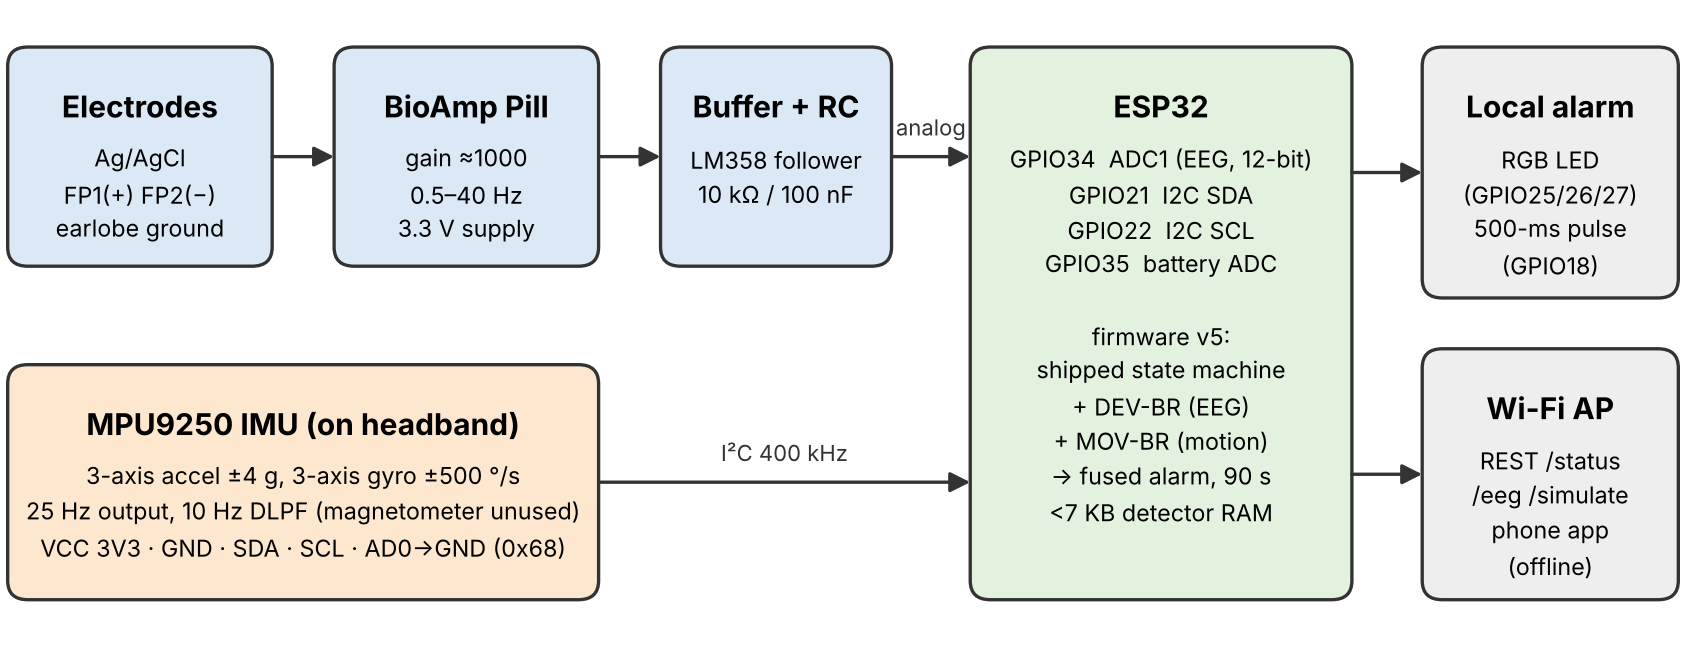
\includegraphics[width=0.86\textwidth]{figures/system_v5.png}
\caption{Prototype (firmware v5). One forehead EEG channel (BioAmp Pill, LM358 follower, RC filter) feeds the ESP32 ADC; an MPU9250 on the headband is read over I$^2$C at 25~Hz. Gain and pass-band are nominal values from the documentation, not measurements.}
\label{fig:hw}
\end{figure*}

\begin{table}[t]
\centering
\caption{Implementation status and source of each specification.}
\label{tab:status}
\footnotesize
\setlength{\tabcolsep}{2pt}
\begin{tabular}{>{\raggedright\arraybackslash}p{0.17\columnwidth}>{\raggedright\arraybackslash}p{0.43\columnwidth}>{\raggedright\arraybackslash}p{0.34\columnwidth}}
\toprule
Item & Specification & Status / source \\
\midrule
EEG front-end & Ag/AgCl FP1$+$/FP2$-$; BioAmp Pill (gain $\approx$1000, 0.5--40~Hz, 3.3~V); LM358 follower; RC 159~Hz & built; nominal values; vendor documents 5-V use~\cite{bioamp} \\
Motion sensor & MPU9250, $\pm$4~g, $\pm$500~$^\circ$/s, 10-Hz DLPF, 25~Hz, I$^2$C GPIO21/22~\cite{mpu9250} & built; not bench-characterized \\
ADC, sampling & 12-bit, default attenuation, \texttt{delay(5)} loop & firmware v5 reports measured rate \\
Outputs & RGB LED, 500-ms GPIO pulse, Wi-Fi AP REST API, phone app & firmware; app not evaluated \\
Detectors & v4: state machine + 3-feature analyzer; v5: DEV-BR, MOV-BR, co-activation & v4 replay-evaluated; v5 compiled (792~KB flash), bit-exact offline \\
Bench / human data & noise, battery, timing, wear & not measured \\
\bottomrule
\end{tabular}
\end{table}

\textbf{Hardware.} One differential forehead channel is amplified by the BioAmp Pill, buffered by an LM358 and digitized by the ESP32; an MPU9250 accelerometer/gyroscope mounted on the headband is read over I$^2$C (Fig.~\ref{fig:hw}, Table~\ref{tab:status}). The device runs from a USB battery bank without galvanic isolation. The LM358 is not rail-to-rail: at 3.3~V its output tops out near 1.8~V, about 150~mV above mid-supply~\cite{lm358}.

\textbf{Shipped detectors (v4).} The firmware tracks a baseline $b[n]{=}0.99\,b[n{-}1]{+}0.01\,x[n]$ and deviation $d[n]{=}|x[n]-\lfloor b[n]\rfloor|$, with an exponentially weighted mean $\mu$ and spread $\sigma$ (forgetting factor 0.995 per sample). Every 30~s it sets BROWNOUT and BLACKOUT thresholds to $\mu{+}2.5\sigma$ and $\mu{+}4\sigma$, clamped to fixed ADC ranges, and leaky counters confirm states. A Python analyzer computes line-length (LL), delta/alpha ratio and 30--45-Hz energy over 2.56~s and requires two of three features above adaptive thresholds on 7 of 8 ticks.

% =============================================================================
\section{Code-Faithful Replay}\label{sec:method}
\textbf{CHB-MIT}~\cite{shoeb2009thesis,goldberger2000physionet} provides the device's exact EEG montage: FP1--FP2 is reconstructed as the signed sum of the bipolar chain from FP1-F7 to FP2-F8 (\NRec{} recordings, \NSz{} seizures, \NHours{}~h, \NSubj{} subjects; chb01 and chb21 are one subject). It has no motion data.
\textbf{SeizeIT2}~\cite{bhagubai2025seizeit2} (CC0) provides \SHours{}~h from \SNSubj{} patients with focal epilepsy recorded in five monitoring units with a wearable: two behind-the-ear EEG channels at 256~Hz and accelerometer/gyroscope data at 25~Hz from a sensor on the back of the neck, the head-borne location closest to our headband. It contains \SNSz{} annotated seizures (\SNFBTC{} focal-to-bilateral tonic--clonic, FBTC; \SNMotor{} focal motor; \SNNonMotor{} focal non-motor; \SNOther{} other). We use the single behind-the-ear channel of each recording (left or right side) as the device's EEG input; \SMovMissing{} of \SNRuns{} recordings lack head-motion data, and there motion detectors cannot fire.

\textbf{Front-end model and replay.} EEG passes a causal model of the nominal pass-band (0.5-Hz high-pass, 40-Hz low-pass), is resampled to 200~Hz, scaled by the nominal gain around 1.65~V and quantized to 12~bits. The analyzer is imported unmodified and driven by a simulated serial port and clock; the firmware \texttt{loop()} is ported line by line. Motion features are computed exactly as in firmware v5 (Sec.~\ref{sec:det}). This is a software replay; no hardware-in-the-loop experiment was performed.

\textbf{Scoring.} Following SzCORE~\cite{dan2025szcore}, alarms within 90~s merge, a seizure counts as detected if an alarm falls in [onset$-$30~s, offset$+$60~s], and other alarms are false alarms (FA). Parameters are selected by leave-one-subject-out cross-validation (LOSO): on all other subjects we pick the most sensitive setting whose pooled FA/h meets a target and apply it to the held-out subject. CIs use a 2000-resample subject bootstrap; detectors are compared per subject with the Wilcoxon signed-rank test, and seizure-level detections with an exact McNemar test. Chance levels come from 200--1000 random circular shifts of each alarm train.

% =============================================================================
\section{Detectors}\label{sec:det}
\textbf{Why the shipped detectors fail.} The firmware's spread estimate forgets within about 1~s, so 4$\sigma$ excursions are routine in ordinary EEG; the analyzer's vote waits on two features that carry no seizure information (delta/alpha AUC \AucDAR{}, high-frequency energy \AucHFE{}); and fixed floors in ADC units make detection gain-dependent.

\textbf{DEV-BR and MOV-BR.} Let $\delta(t)$ be the per-second mean of the firmware deviation $d$, and $\alpha(t)$ the per-second mean of $\lVert \mathbf a - \mathrm{EMA}_{1\,\mathrm s}(\mathbf a)\rVert$ for the 25-Hz acceleration $\mathbf a$. For either signal $s$,
\begin{equation}
\rho_s(t) = \log \frac{s(t)}{\operatorname{median}\{s(\tau): t{-}329 \le \tau \le t{-}30\}},
\end{equation}
so each wearer is compared with their own background 30--330~s earlier and the units of the sensor cancel. A condition holds when $\rho \ge \log r$ for $D$ consecutive seconds; MOV-BR may also require that 2--7~Hz power (Hann window, last 4~s) exceed a share $q$, as in clonic jerking. The \emph{general mode} raises an event when the EEG \emph{or} the motion condition starts; the \emph{convulsive mode} raises an alarm when $\rho_\delta \ge \log r_E$ \emph{and} $\rho_\alpha \ge \log r_M$ hold together for $D$ seconds. Each output fires at most once per 90~s and not before 330~s.

\textbf{Firmware v5.} The general event drives the existing BROWNOUT warning and the convulsive alarm drives BLACKOUT (red LED, GPIO pulse, app); the v4 serial format is unchanged. The detectors hold two 330-value histories and use \texttt{std::nth\_element} once per second (5~KB), plus 1.6~KB for motion features; v5 compiles for the ESP32 at 792~KB flash (v4: 767~KB). Its parameters are the modal LOSO choices: general mode $r{=}2$, $D{=}20$~s for EEG, $r{=}24$, $q{=}0.4$, $D{=}20$~s for motion (\SFusAParamsN{}/125 folds); convulsive mode $r_E{=}4$, $r_M{=}8$, $D{=}30$~s (\SCvAParamsN{}/125 folds). On the host, the C++ code matched the Python motion features to float precision and reproduced every alarm of the evaluation \SVerNote{}. It has not yet been timed on the ESP32.

% =============================================================================
\section{Results}\label{sec:res}
\begin{table*}[t]
\centering
\caption{CHB-MIT, FP1--FP2 (\NSubj{} subjects, \NSz{} seizures, \NHours{}~h; nominal front-end). Brackets: subject-bootstrap 95\% CI. ``Macro'': mean of per-subject sensitivities. ``Chance'': sensitivity of randomly circularly shifted alarms. BR rows: held-out subjects (LOSO).}
\label{tab:chb}
\begin{tabular}{lcccccc}
\toprule
Detector & Detected & Sensitivity [95\% CI] & Macro & FA/h & Latency (s) & Chance \\
\midrule
\MainTableBody
\bottomrule
\end{tabular}
\end{table*}

\begin{table*}[t]
\centering
\caption{SeizeIT2 (\SNSubj{} patients, \SNSz{} seizures, \SHours{}~h; behind-the-ear EEG through the device model, head-borne accelerometer). All non-firmware rows: held-out patients (LOSO). Class columns give the share of seizures of that class detected; ``Sleep'': seizures annotated as arising from sleep.}
\label{tab:s2}
\small
\setlength{\tabcolsep}{4pt}
\begin{tabular}{lcccccccc}
\toprule
Detector & Detected & Sensitivity [95\% CI] & FA/h & FBTC & Focal motor & Focal non-motor & Sleep & Chance \\
\midrule
\SMainTableBody
\bottomrule
\end{tabular}
\end{table*}

\begin{figure}[t]
\centering
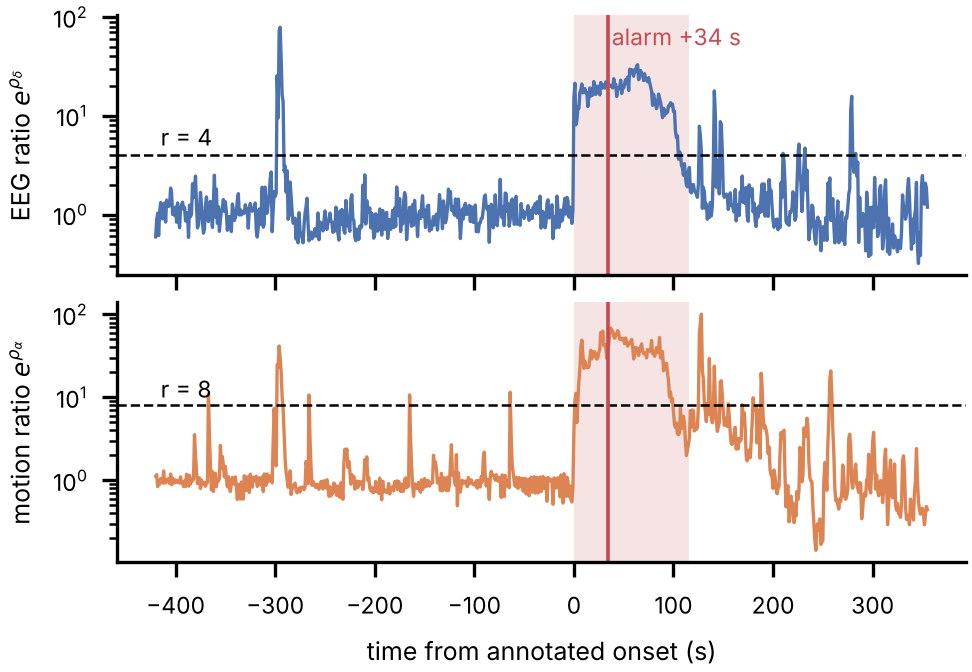
\includegraphics[width=0.95\columnwidth]{figures/convulsive_example.png}
\caption{Convulsive-mode alarm on an FBTC seizure (shaded) in SeizeIT2 patient 115, arising from sleep. Brief EEG artifacts and isolated movements cross one threshold but not both; the seizure raises both ratios and the alarm fires after the 30-s persistence. Shown: the detected sleep FBTC seizure with the shortest latency and no false alarm within 30~min (illustrative, not typical).}
\label{fig:example}
\end{figure}

\begin{table}[t]
\centering
\caption{CHB-MIT front-end robustness (simulated). ``Fixed'': DEV-BR with $r{=}\HwFixR$, $D{=}\HwFixD$~s chosen at gain 1000. Clip: LM358 1.8-V ceiling; Sat.: saturated samples. Cells: sensitivity / FA/h.}
\label{tab:hw}
\footnotesize
\setlength{\tabcolsep}{1.5pt}
\begin{tabular}{lcccc}
\toprule
Condition & Sat. & DEV-BR fixed & DEV-BR LOSO & Firmware \\
\midrule
\HwTableBody
\bottomrule
\end{tabular}
\end{table}

\begin{figure}[t]
\centering
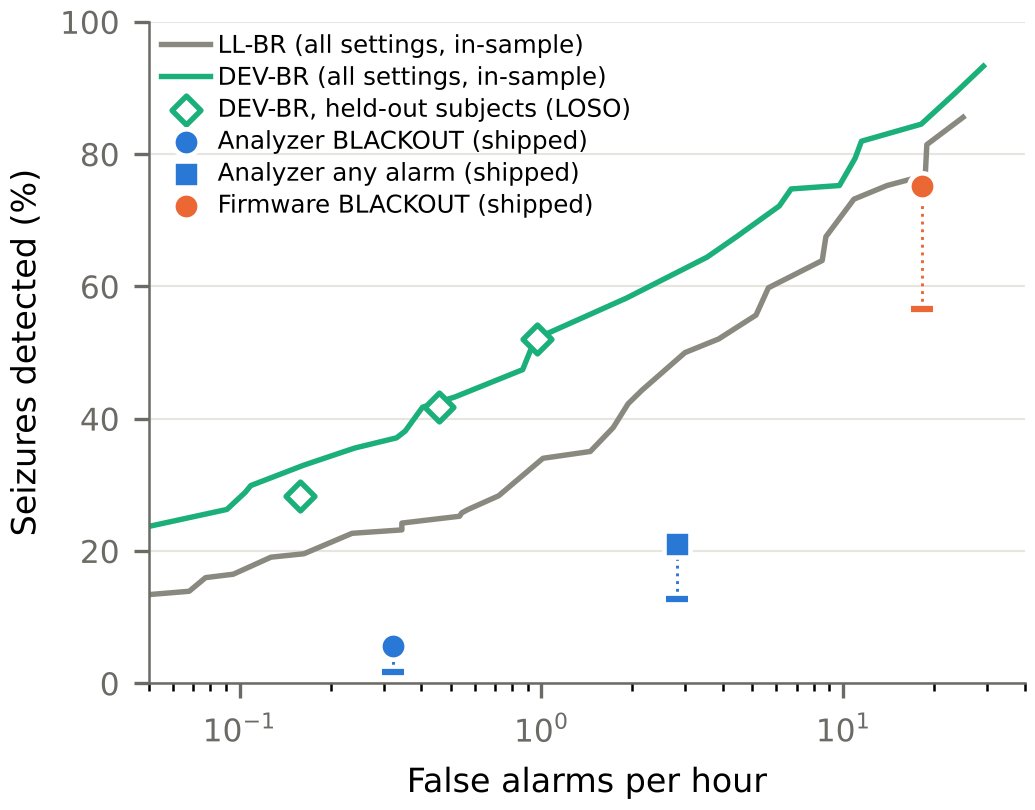
\includegraphics[width=0.88\columnwidth]{figures/operating_curve.png}
\caption{CHB-MIT, FP1--FP2: sensitivity versus FA/h. Lines: best in-sample ratio trade-offs; diamonds: DEV-BR on held-out subjects; markers: shipped detectors, with dashes at their chance levels.}
\label{fig:roc}
\end{figure}

\textbf{CHB-MIT (device montage, EEG only).} The analyzer's BLACKOUT alarm detected \PyBSens{} at \PyBFAh{}~FA/h; the firmware reached \FwBSens{} at \FwBFAh{}~FA/h, but randomly shifted copies of its alarms already reach \FwBNull{} (Table~\ref{tab:chb}). DEV-BR detected \DevADet{}/\NSz{} seizures (\DevASens{}, CI \DevACI{}) at \DevAFAh{}~FA/h with a median latency of \DevALat{}~s (Fig.~\ref{fig:roc}), about \FoldDevPy{} times the analyzer at a comparable alarm rate. It was better in \TestDevPyBetter{} of \TestDevPyN{} subjects and worse in none (\TestDevPyP{}), against a chance level of \DevANull{}. Without normalization the same procedure reached \AblAbsSens{}, and logistic regression and boosted trees on 14 normalized features did not do better (best \AltBestOneSens{} at $\le$1~FA/h). With parameters frozen, DEV-BR stayed at \HwDevSensMin{}--\HwDevSensMax{} and \HwDevFAMin{}--\HwDevFAMax{}~FA/h across gains of 500--2000, LM358 clipping, a 3.1-V ADC range and a 6-ms loop, while the firmware moved between \HwFwSensMin{} and \HwFwSensMax{} at \HwFwFAMin{}--\HwFwFAMax{}~FA/h (Table~\ref{tab:hw}; simulation).

\begin{figure*}[t]
\centering
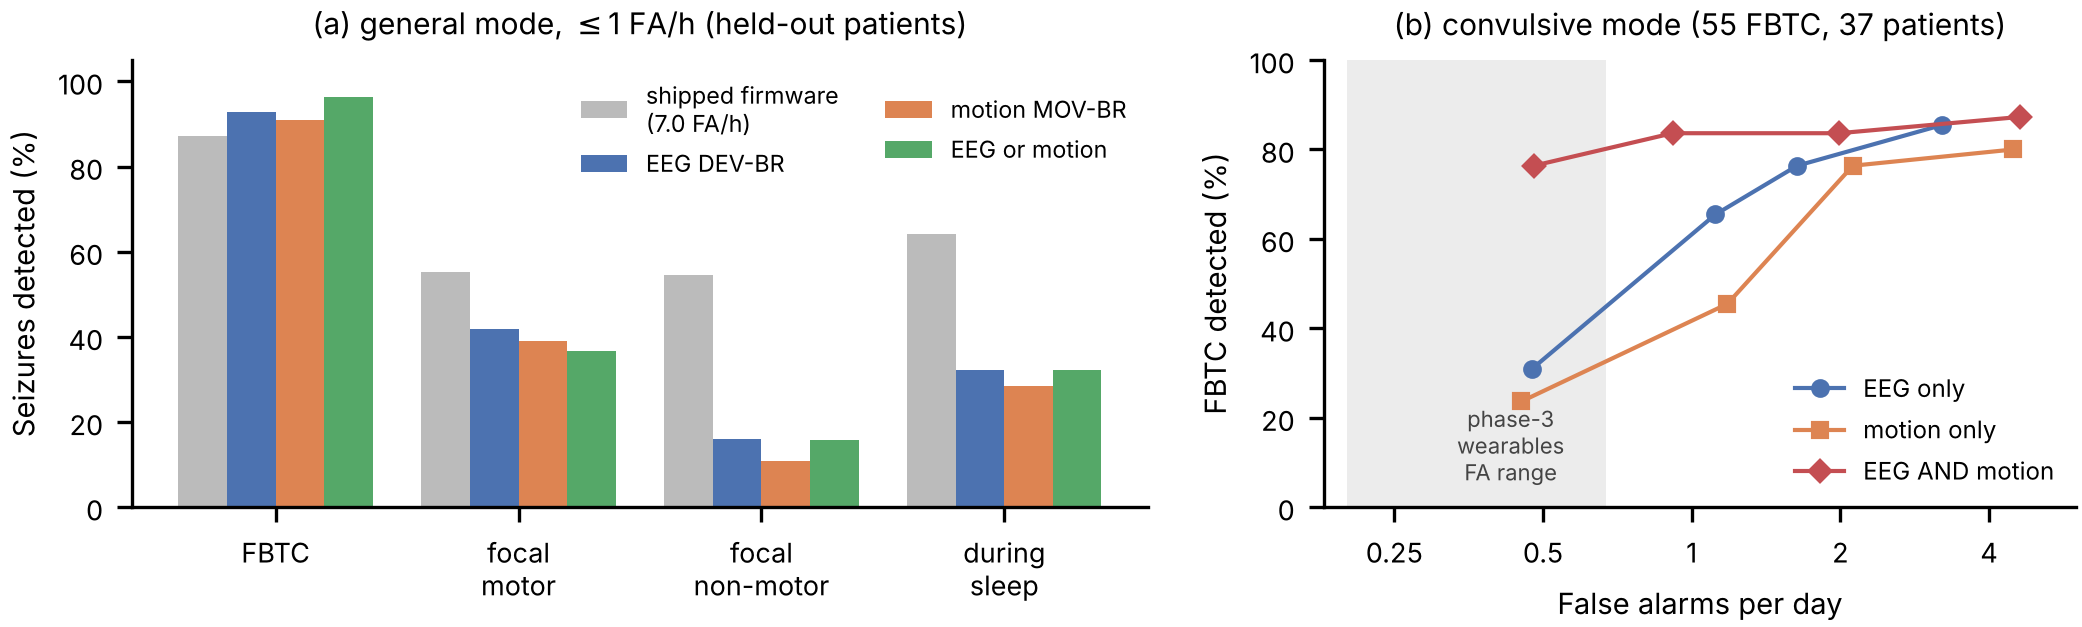
\includegraphics[width=0.92\textwidth]{figures/seizeit2_results.png}
\caption{SeizeIT2, held-out patients. (a) Share of seizures detected by class at $\le$1~FA/h (the shipped firmware at its own 7.0~FA/h). (b) Convulsive mode: FBTC sensitivity versus false alarms per day for LOSO targets of 0.02--0.2~FA/h; shaded, the range reported for phase-3 wearables~\cite{beniczky2021guideline}.}
\label{fig:s2}
\end{figure*}

\textbf{SeizeIT2: shipped firmware and general mode.} On behind-the-ear EEG the shipped firmware detected \SFwSens{} at \SFwFAh{}~FA/h (\SFwFAday{} per day), against a chance level of \SFwNull{} (Table~\ref{tab:s2}). At the same alarm rate, EEG-or-motion detected \SFusFwSens{} (\STFUSEDFwVFWBetter{} patients better, \STFUSEDFwVFWWorse{} worse, \STFUSEDFwVFWP{}) and DEV-BR alone \SEegFwSens{}. At $\le$1~FA/h, DEV-BR detected \SEegASens{} (macro \SEegAMacro{}; chance \SEegANull{}), MOV-BR \SMovASens{}, and their combination \SFusASens{}: motion detected seizures the EEG missed but added as many false alarms, so the general mode did not beat EEG alone (\STFUSEDAVEEGAP{}). Gyroscope magnitude was weaker than acceleration (\SGyrASens{}), and a rhythm gate was selected in every MOV-BR fold. Detection depended strongly on seizure type (Fig.~\ref{fig:s2}a): \SFusAFBTC{} of FBTC seizures, \SFusAMot{} of focal motor and \SFusANonMot{} of focal non-motor seizures.

\textbf{SeizeIT2: convulsive mode.} Requiring EEG and head motion to rise together removed most false alarms from ordinary movement and from EEG artifacts. With parameters chosen for FBTC seizures at $\le$0.02~FA/h, co-activation detected \SCvADet{}/\SCvAN{} FBTC seizures in \SCvASubj{} patients (\SCvASens{}, CI \SCvACI{}) at \SCvAFAday{} false alarms per day, including \SCvASleepDet{} of \SCvASleepN{} that arose from sleep (Fig.~\ref{fig:example}); \SCvAZeroFA{} of 125 patients had no false alarm. At the same rate, EEG alone detected \SCvEegSens{} and motion alone \SCvMovSens{} (co-activation found \SMcEegOnly{} FBTC seizures that EEG missed and missed \SMcEegOther{}, \SMcEegP{}; versus motion, \SMcMovOnly{} and \SMcMovOther{}, \SMcMovP{}; Fig.~\ref{fig:s2}b). With a 0.05-FA/h target it detected \SCvBSens{} (CI \SCvBCI{}) at \SCvBFAday{} false alarms per day. The median latency was \SCvALat{}~s (IQR \SCvALatIQR{}) from the annotated focal onset, which precedes bilateral spread.

% =============================================================================
\section{Discussion and Limitations}
Replaying the code that ships showed that the prototype's original alarms mostly fire at random, and that one rule---compare a signal with the wearer's own delayed median---fixes this for EEG and transfers to a motion sensor without knowing its units. Adding the MPU9250 changed the outcome for the seizures that matter most for safety: neither modality alone reached a usable false-alarm rate, but their co-activation detected about three in four convulsive seizures at a rate inside the range of phase-3 wearables, with under 7~KB of RAM and no machine learning. Three principles generalize: validate the shipped code, not a re-implementation; normalize against the wearer's own background so decisions do not depend on sensor units or gain; and fuse modalities with \emph{and} when the target event moves both.

The absolute performance still falls short. Clinical wearables reach 90--96\% for tonic--clonic seizures~\cite{beniczky2021guideline}, and a learned multimodal model on SeizeIT2 reached 95.5\% at 1.1 false alarms per day~\cite{zhang2024multimodal}; focal non-motor seizures were rarely detected at a usable rate. Limitations: (i)~all results come from software replay; no recordings from the prototype, bench measurements of the MPU9250 or front-end, or human tests are reported. (ii)~SeizeIT2 differs from the device: its EEG is behind-the-ear rather than FP1--FP2, its motion sensor sits on the neck at 25~Hz rather than on the headband, and it was recorded in hospital. (iii)~The front-end model uses nominal values; non-idealities were simulated, not measured, and the BioAmp runs below its documented supply. (iv)~FBTC results rest on \SCvAN{} seizures from \SCvASubj{} patients. (v)~v5 parameters are modal LOSO choices from the same data, and v5 has not been timed on the ESP32. Next steps are bench characterization, overnight recordings with the headband, and an ethics-approved study.

% =============================================================================
\section{Conclusion}
We built a low-cost EEG and head-motion seizure alarm and evaluated its code as shipped on two public datasets, \NSubj{} and \SNSubj{} patients. The shipped detectors fail for identifiable reasons. A delayed-median ratio rule fixes the EEG detector (\DevASens{} at \DevAFAh{}~FA/h on the device montage, robust to front-end errors), and requiring EEG and motion to agree detects \SCvASens{} of convulsive seizures at \SCvAFAday{} false alarms per day, in firmware that fits in under 7~KB of RAM. Hardware, firmware, analyzer, replay benchmark and detectors are released for others to reproduce and extend.

\section*{Data and Code Availability}
CHB-MIT~\cite{goldberger2000physionet} and SeizeIT2~\cite{bhagubai2025seizeit2} are public. Firmware (v4 and v5), analyzer, schematics, replay code and the C++ detectors are at~\cite{vera_repo}.

\section*{Acknowledgment}
The authors used an AI assistant (Claude, Anthropic) to help develop the evaluation code and firmware and to draft the manuscript; the authors reviewed all content and take full responsibility for it.

\bibliographystyle{IEEEtran}
\bibliography{refs}

\end{document}
